\documentclass[a4paper, 12pt]{article}
\usepackage[utf8]{inputenc}

\title{Social Comparison and Cooperation: An Experimental Approach}
\author{Felipe Galera Mart\'inez}
\date{\today}
\usepackage{hyperref}
\usepackage{natbib}
\usepackage[toc,page]{appendix}
\usepackage[dvipsnames]{xcolor} % Letras de colores
\usepackage{float} % to anchor figures
\usepackage{amsmath} % split equations
\usepackage{graphicx} % for the tables
\usepackage{booktabs} % for the tables
\usepackage{anysize} % necessary for the command "marginsize"
\marginsize{4cm}{2cm}{2.5cm}{2.5cm} % format of the page
\bibliographystyle{agsm}
\providecommand{\keywords}[1]{\textbf{\textit{Keywords---}}#1} % To introduce keywords
\renewcommand{\baselinestretch}{1.5} % line spacing 1.5
\addtolength{\skip\footins}{2pc plus 5pt} % change the footnote to the text distance
% \renewcommand{\thesection}{\Roman{section}}  % roman numbers in sections
% \renewcommand{\thesubsection}{\thesection.\Roman{subsection}}  % roman numbers in subsections


\begin{document}
\maketitle
\thispagestyle{empty}
\begin{abstract}
This paper proposes an laboratory experiment to investigate the impact of social comparison and fairness in cooperation. I consider a two-person public good game with heterogeneity in the subjects' endowment distribution. Some workers receive homogeneous pay-rate (fair wages), while other workers receive unjustified heterogeneous pay-rates (unfair wages). I proposed an empirical strategy to check plausible hypothesis derived from the literature and from the main social preferences models. The main testable predictions are that: (i) participants cooperate more if they have a higher salary, (ii) participants cooperate less if they face unequal wage distribution and, (iii) participants cooperate less between each other if they have different unjustified salaries. 


\end{abstract}
\keywords{ Labor market experiments, Real effort, Social comparison, Wage schemes, Cooperation, Public goods}

\newpage
\tableofcontents
\thispagestyle{empty}
\newpage

\setcounter{page}{1}
\section{Introduction}

Payoff and fairness comparisons across workers at firm level is inevitable, as usually workers share the same work environment and interact with each other. These situations reveals the nature of social comparisons and how our perception of fairness affects workers morale, and therefore productivity \citep{Loewenstein2000, NBERw18687}. Even if these comparison schemes do not come from the workers initiative, policy makers are actively trying to tackle the idea of "equal pay for equal work" as reflected in the Non-Retaliation Executive Order from the White House in 2014 (E.O. 13665 of Apr 8, 2014), or recently in Europe in the new 2018 law on wage transparency in Germany. The final goal of this policies is promoting the idea of abolishing pay secrecy, making easy to spot salary discrimination between workers (being gender or race reasons the more salient ones).

A potential concern using a non-laboratory setup to study the effect of horizontal fairness on cooperation is that is hard to disentangle the different mechanisms by which this effect can take place. Shared values \citep{Ostrom2000} or asymmetry of information between the workers \citep{Cardenas2003} are two salient examples of potential influencers of workers cooperation level between each other’s. I propose a controlled lab design in which participants play a real-effort task followed by a classic cooperation game, a one-shot Public Good Game.

The remaining of the paper is structured as follows: Section 2 introduces a literature review of laboratory experiments related with peer-comparison and reference-dependent preferences, focusing in the ones related to wage fairness and cooperation. Section 3 presents the experiment design. Section 4 explains the estimation strategy. Section 5 examines different theoretical models and the hypotheses based on them. Section 6 concludes the paper. 

\section{Literature Review}

This paper contributes to the literature of laboratory experiments on the effect of horizontal comparison and fairness preferences. A small number of experiment, both in laboratory and in a field setup, pursue a direct horizontal comparison between workers’ on productivity with real effort tasks \citep{Greiner2011, Cohn2014, Azmat2015}. The aim of the paper is taking the experimental methodology of this research line, but proposing the potential effects of peer-comparison on cooperation instead of labor supply as the variable of interest. 

While \citep{Charness2007} put on relevance the lack of evidence that work effort is affected by coworkers wages, a new and growing field emerge since then (.e.g., \cite{Greiner2011}; \cite{Kube2012},\cite{Ku2013},\cite{Cohn2014}, and \cite{CohnFehr2014}, find a significant effect of reference-dependent preferences). The essence of reference-dependent preferences was theorized by \cite{Akerlof1990} in their fair wage-effort model, in which it stress the importance of horizontal comparisons and fair considerations among employees. In the model, individuals take other peers as a reference point and shape their consideration of what is their own fair wage. Later experiments related to reference-dependent preferences show that workers’ salaries are partly judged by their peers-salaries.

The link of fairness and reference-dependent preferences is explored in \cite{Gachter2012}, that investigates the effect of worker comparisons for workers productivity. The authors use a three-person gift-exchange game, one employer and two employees, in three studies. In the first study, the game is played eight times and they randomly re-match the group of three players every period. The workers that face disadvantageous wage discrimination, not justified by circumstantial differences or merit, significantly reduce their effort relative to a situation with equal wages. 

In the second study they take into account individual preferences, as different effect directions might cancel each other out in the aggregate. In this case, the workers choose their effort before they know their wages set by the employer. While the size of the wage discrimination effect is not as strong as in other previous studies, on average people react negatively to disadvantageous wage differences.  

The third study explores the fairness concerns of the players, as the differences in the effort could have been caused by intentional wage discrimination or due the payoff differences. If the employer is not responsible for the discrimination, there is no clear reason to punish her for the wage inequality. 
  
Another experiment showing peer-comparison is \cite{Bracha2012}, in which they explore the impact of heterogeneity in wages on labor productivity. In this laboratory experiments participants solve 4x4 matrix that exactly sum to 10 for a given pay rate. After a training round, they are asked if how long they want to work on the task, from 0 up to 30 minutes. In the control treatment, half of subjects receive \$0.40 and the other half receive \$0.80, both types only aware about one pay-rate (their own). 

In other treatment, subjects face the same matrix task with the same pay-rates but in this case, they are informed of the relative pay differences for the same tasks. When peer-comparisons is available, the lower paid participants (\$0.40 per matrix) significantly choose to work less time and solve less matrix within the time elected than in the group with no relative pay-rate information available.
 
To investigate the mechanism behind the information treatment they create two conditions, both using an essay evaluation before the main matrix task. For the first condition the subjects are asked to write a short essay up to 200 words before the experiment about their previous day’s lunch experience. Then, in the experiment session, the subjects have to count the number of r’s is written in their essays and they are informed that the pay-rate in the matrix task depend on their performance. Those with a r count higher than the median receives the higher wage (\$0.80 per matrix), being informed one by one privately by the experimenter. Those with low pay-rate supply less labor than their equals in the control treatment with no information but it does not affect the performance of high pay-rate subjects significantly. This empirical fact is consistent with \cite{ Fehr1999} as disadvantageous inequality is more painful for the subjects than for advantageous inequality.
 
For the second condition, they include a stronger justification for the wage disparity. The experimenters already made a pre-written essay for which the subjects have to count the number of r’s as in the first condition. In this study participants are informed that the experimenter evaluation of their counting performance would determine their pay-rate assignment, but the experimenter do not explain how in an intentionally ambiguous way. Again, those with a r count higher than the median receives the higher wage. The regression analysis suggests that the relative pay effect on labor supply disappear when the subjects feel that their pay-rate is link to their actual performance, showing that fairness of pay is a determinant of labor supply.

Both \cite{Gachter2012} and \cite{Bracha2012} disclose worker reference-dependent preferences, and the effect on labor supply. Also, and in line with the purpose of this paper, they reveal that workers not only care about the differences in pay-rates but also about the fairness and reasons behind the wage differences. When the pay-rates seems more justify for the participants, the effect of pay disparity on work effort disappear or lose strength. 

These papers have a ground in the theoretical framework about fairness comparisons, being \cite{Fehr1999} the most notorious reference. The model assumes that people care about other people' fair payoffs, and therefore comparisons between agents are included in their utility function. In short, people have what it's broadly known as social preferences for fairness. This is a central assumption for this experiment, that is widely proven in economic experiments (e.g. \cite{ferguson2016} for a meta-analysis). Also, latest medical studies have proven that thinking about different types of allocation of resources (reciprocal, fair, unfair)  between people triggers brain activity in charge of moral consideration (see \citep{niemi2017sees, Niemi2017}). Although the concept of a fair allocation varies depending on the context of the decision, the sense of fairness is probably a human universal \citep{Henrich2001}. 

In relation with the second part of this experiment proposal, \cite{BUCKLEY2006} examines the effect of endowment wealth heterogeneity on cooperation. In this experiment individuals are randomly arranged into groups of four and play a public goods game 10 times. In each round they receive a certain amount income player and decide to a allocate part of this income into a private or a group account. The rate of conversion is one to one token if they allocate into the private account (the full amount), and one to half token if the allocate into the group account (half of the token to each of the four players in the group). The income is heterogeneous among the participants and is shown to them as part of the feedback in every round to make more salient the social peer-comparison. 

Following \cite{Fehr1999} reasoning, the individuals with the lower income should contribute less than higher income as the parameter for disadvantageous inequality is straightly more than the parameter for advantageous inequality. The authors find that the participants with low income contribute a higher percentage of their income to the public good, in contrast with inequality-aversion \cite{ Fehr1999} model. As an alternative explanation, they propose that this behavior could be due to the participants feel that they must contribute what they consider a fair share to the public good, independent of their income \citep{Sugden1984}. That could explain why the participants tend to contribute one-fourth the amount that the entire group contributes, and not proportionally to their income.

\cite{Spiller2016} conducted a one-shot public good game experiment with asymmetric endowments in which they create "poor" and "rich" players artificially. Once the players receive the endowments, they elect different normative beliefs about what they think is they right amount to contribute, and different expectations about what others will contribute. Rich players contribute a more in relative terms than Poor players, in contrast with the previous mentioned article \citep{BUCKLEY2006}

In relation with the literature above mentioned, this experiment combines fairness and reference-dependent preferences with contribution of common one-shot public good.

\section{Experiment Design}

I present a individual real effort task followed by a two-person public good game to explore the effect of heterogeneity in the distribution of endowments on conditional contribution. Consistent with \cite{OXOBY2013}, the one-shot and two players design looks for the simplest possible cooperation environment. The participants are framed in the game as workers, and the contribution to the public good as a cooperative business decision. This framing mask the public good game in a credible firm real-life decision in which two parts have to contribute to create a possible win-win situation.

\subsection{Stages}

In the first stage of the experiment, each worker $i \in (1,n$) play a real effort-task that consist in a 3x3 matrix with different quantities (see Appendix 1. Instructions Stage 1). In each cells participants have to try to use to sum ten. The stage consists in twenty rounds of one minute of duration with nine matrices to solve (which is hardly doable). To ensure the correct understanding of the rules and to familiarize the participants with the game, they are asked to answer four control questions ([Control Questions A. Stage 1.]) and play a round of 1 minute of the matrix-game without payoffs before the proper game with real consequences takes place. 

Moreover, workers are informed that they will play a second stage in which they can use their total earnings $e_i \in (0,n$) from the first stage to might earn more in a second stage (Public Goods Game), but they are not informed that the second stage consist in a cooperation game in order to avoid strategic behavior or influence the effort in the first stage. Once every worker is done working on the matrix task, they start the second stage. In the second stage the workers are randomly matched together in groups of two $i_i \in (1,2$), and they have the possibility to make a cooperative business together investing some of their earnings $c_i \in (0,n$). Their final payoffs are given by:

\begin{equation}
\prod_i(c_i,c_j) =  (e_i - c_i) + 0.75\cdot (c_i + c_j), \quad i\neq j \quad \quad
\end{equation}

Finally, once the experiment is over, subjects fill out a questionnaire (see Appendix 3. Final Questionnaire). I use these demographic data as controls for the regression analysis. 

\subsection{Treatments}

Workers are randomly assigned to one of two treatments. In the "fair wages" treatment, all workers in a single session have the same pay-rate per correctly solved matrix. This pay-rate, 2 Danish krones per matrix ($w_M =2$), is common knowledge as is stated in the instructions and they are read out loud by the experimenter during the session. 
On the contrary, in the "unfair wages" treatment the workers receive heterogeneous pay-rates changing the are pay-rate distribution. Workers are randomly assigned to a denoted High Wage, Medium Wage or Low Wage ($w_L= 1, w_M = 2, w_H= 3$), that are also common knowledge as is stated during the session both by the instructions and the experimenter. 

The formation of groups of two workers with identical tasks made it very plausible that the two workers became natural comparison agents for each other, making salient the peer-comparison between them. This one-time Public Goods Game, in contrast with a repeated contribution game, does not grant the possibility of developing trust or direct reciprocity between workers. The one-time setup determines the indirect reciprocity effect towards the experiment distribution of wages (that the workers are not responsible of). In any repeated cooperation game design, this effect could be easily underwhelmed by the reciprocity towards the peer-workers. 

This is it, the participants could be responding friendly or hostile actions to the last action of their peer, and not because the unfair treatment in wages. For one-time only cooperative decisions, the workers do not have the opportunity to reward or punish actions towards each other. 

\section{Estimation Strategy}

For the estimation strategy I propose an extension of \cite{SPRAGGON2009} regression analysis, in which cooperation is proxied as percent aggregate contribution. For my experiment, there are two types of workers pairing denoted in terms of "own wage/other's wage": 

both workers have the same wage (Low/Low, Medium/Medium, High/High), or workers have different wages (Low/Medium, Low/High and vice versa). 

For the fair wage treatment there are only the former type of workers, given that they face the same wages, while in the unfair wage treatment there is mixed matching.
I propound examining the effect of relative pay differences using OLS:

\begin{equation}
\begin{aligned}
c_i/e_i =\quad  &  \alpha + \beta_1(w_i^L/w_j^L) + \beta_2(w_i^M/w_j^M) + \beta_3(w_i^H/w_j^H)\\
                & + \beta_4(w_i^L/w_j^H) + \beta_5(w_i^M/w_j^H) + \beta_6e_i + \beta_7e_j\\
                & + \beta_8Treatment\cdot(w_i - w^H) + \beta_9Treatment\cdot(w_i - w^L)\\
                & + \beta_{10}X_i + \varepsilon_i
\end{aligned}
\end{equation}

Heeding \cite{SPRAGGON2009} original idea, the regression measure the aggregate contribution to the project as a percentage of the total earnings ($c_i/e_i$), given the different possible relative pay combinations ($\beta_1 - \beta_5$) and the total earnings of the workers ($\beta_6 - \beta_7$). 

However, the extension includes an envy coefficient ($\beta_8$) and an altruism coefficient ($\beta_9$). As in \cite{Fehr1999}, envy measures the utility loss from the disadvantageous wage inequality, while altruism parameter measures the utility loss from an advantageous wage inequality. 

Notice that some parameters are only available in the unfair treatment given that in the fair treatment the wages are homogeneous ($w_M=2$) and therefore, no social comparison or relative standing mechanism takes place. For example, if random matching pair two workers with low wages, altruism parameter should not take place ($\beta_9$ = 0), but the workers still know that they are different distribution of wages and might be "envious" (Testable $\beta_8$ \neq 0)

Lastly, ${X_i}$ is a vector of covariates that includes gender, foreign, age and their own consideration of quantitative skills (Appendix 3. Final Questionnaire). These extended controls, in my opinion, are necessary for avoiding omitted variables problem. For example, \cite{Gneezy2003} and \cite{Bracha2012} found that women and men behave differently in competitive and cooperative context. Math task like the used matrix summatory task could create anxiety \citep{Ashcraft2001, Keogh2001} and therefore, influence the level of cooperation. Also, people inherent ability solving quantitative problems could affect their decisions in social dilemmas games \citep{Lezzi2015}. 

\section{Theoretical Models and Hypothesis}

These hypotheses build on the above-mentioned research, and according to three models selected that tackle deviations of self-interest behavior. 

The first type of model test the \textit{Income Effect} on cooperation. \cite{Becker1974} propose a simple model in which the utility functions of the participants depends on the participants’ own total wealth, and it is increasing on the wealth of other group members:
\begin{equation}
\begin{aligned}
U_i &= f(e_i, R(e_j)), \quad i\neq j \quad \quad
\end{aligned}
\end{equation}
Where R is the perception of i held by other persons. In the context of the experiment, R is function of their relative income. The model predicts that workers with high wages will cooperate more than workers with low wages (See \cite{BUCKLEY2006} for the math proof). \\

\textbf{Hypothesis 1}: Workers cooperate more if they have a higher marginal monetary payoffs. (\textit{Income effect}) \\

This first hypothesis is testable in my estimation strategy by checking $\beta_6 = 0$ and  $\beta_7 = 0$. The second model by \cite{Fehr1999} consider inequality-aversion, and test the \textit{Unfairness Effect} on cooperation. This model describes certain situation were there is a fraction of self-interested people and another fraction of people that care about inequality of outcomes and are motivated by fairness considerations. In their two-player setup the utility function is determined by the distribution of income among the players: 
\begin{equation}
\begin{aligned}
U_i &= w_i - \alpha_i \underbrace{max\{w_i-w_j,0\}}_\text{Envy parameter} - \beta_i \underbrace{max\{w_j-w_i,0\}}_\text{Altruism parameter}, \quad i\neq j \quad \quad
\end{aligned}
\end{equation}
Where $w_i$ is the own pay-off, the \textit{envy parameter} represents the disutility of advantageous inequality and the \textit{altruism parameter} represents the disutility of disadvantageous inequality.\\

\textbf{Hypothesis 2}: Agents contribute less share of their income level if they notice that they are being paid differently for the same exact task. (Unfairness effect) \\

This second hypothesis is testable in my estimation strategy by checking if $\beta_8$ and $\beta_9$ are statistically different from 0. Lastly, I consider \cite{Bolton2000} model that is constructed on the basis that people are motivated by their own pay-offs and their relative standing pay-offs (ERC or Equity, \textit{Reciprocity, and Competition} model). \\

\textbf{Hypothesis 3}: On average, workers lower their cooperation towards each other if they are matched with an unequal better paid partner. (Social Comparison effect)\\

This last hypothesis is testable by checking the difference in average aggregate contribution between equal Medium Wage matched partners ($\beta_2$) in fair and unfair treatment.


\section{Conlusion}

I consider a laboratory experiment to study the effect of fairness concerns and social comparison on cooperation level. Participants work on a first stage real-effort task, a battery of 3x3 problem matrices, in which they face homogeneous pay-rates (fair wages treatment) or heterogeneous pay-rates (unfair wages treatment). Participants then cooperate in a one-shot two-player Public Good Game, framed as a common Project. The estimation strategy aims to test if unfairness in the distribution of the wage's triggers spillover effect towards lower cooperation between workers, an idea supported on both theoretical and empirical grounds. 
\begin{appendices}

The instructions are intended to be concise and avoid stating any positive externality associated with public goods to not affect contributions by the word’s selection. The text follows the instructions design advices of \cite{Ramalingam2016}, adapted to my experiment. Instructions for Stage 1 are read out loud by the experimenter. Same for Instructions for Stage 2, once every participant had finish Stage 1 and the experimenters already handed the printed instructions.

The only difference between \textcolor{Green}{Fair Treatment} and \textcolor{Red}{Unfair Treatment} instructions is in Stage 1, and it is stated in different colors (Green for Fair, Red for Unfair) to prevent over text.

\chapter{\textbf{Appendix 1. Instructions Stage 1.}}

Welcome to our experiment. No talking, looking around or using your phone is allowed. If you violate any of these restrictions we might ask you to leave the experiment without getting paid. Please, feel free to raise your hand and one of us will assist you if you have any question or anything is unclear at any point in the experiment. 

This experiment is about decision-taking. You will receive 50 Danish kr. for showing up on time. Additionally, if you follow the instructions correctly, you can earn more money depending on your own decisions and on the decisions of others. All participants faces the same set of decision tasks. Everything you earn will be for you and paid in cash in a private way at the end of the experimental session. Your decisions are private and no other participant will know about them. All your data is keep strictly confidential.

Notice that all the instructions are also stated in your computer screen. Please remember to press continue button when you finish reading, and understanding, the instructions.

\begin{center}
\textbf{Stage 1}
\end{center}

The experiment consist in two stages. For the second stage further instructions will be provided. The first stage consists of 20 consecutive rounds of 1 minute. In each round you will face 9 matrices of 3x3 as the one below:

\begin{figure}[H]
\centering
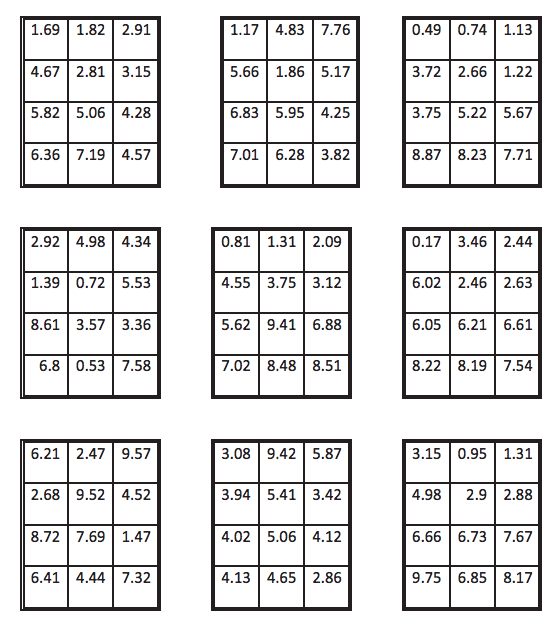
\includegraphics[width=\textwidth,height=11cm,keepaspectratio]{figure_2.png}
\end{figure}

In each matrix you should look for a set of numbers that sum up exactly to 10. When you find a pair of number that adds 10, select the corresponding numbers as highlighted in the image below:

\begin{figure}[H]
\centering
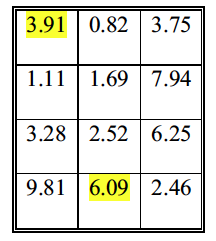
\includegraphics[scale=0.6]{figure_1.png}
\end{figure}

Therefore, you will have 20 minutes to complete the task. \textcolor{Green}{[You will receive a salary of 2 Danish kr. for every matrix solved correctly]}*. Please press continue. Your total earnings will be the sum of your earnings from all of the 20 rounds.

Once the 20 minutes is up, you will receive the feedback of your the amount of matrices solved and your correspondent total earnings. Please answer the following questions and, when you finish, wait patiently. 

\begin{center}
*PLEASE, FOR \textcolor{Red}{UNFAIR TREATMENT} SUBSTITUTE FOR:
\end{center}
\textcolor{Red}{[You will receive a salary for every matrix solved correctly. There are different salary rates. You will be randomly selected to either have a salary of 1 Danish kr. per solved matrix correctly, 2 Danish kr per solved matrix or 3 Danish kr per solved matrix. This salary rate is indicated at the following screen (press continue button). Your salary is fix during the entire game]}.

\begin{center}
\textbf{[Control Questions A. Stage 1. \textcolor{Green}{Fair Treatment}]}
\end{center}

1. “How much have to add-up the selected cells of the matrix to be considered a correct solved matrix?”
\begin{center}
Sol: 10
\end{center}
2. “Suppose that you end up solving 67 matrices correctly at the end of the 20 minutes. What would be your earnings, in krones, for this stage?” \\
\begin{center}
Sol: 134
\end{center}
3. “Suppose that you end up solving 76 matrices correctly at the end of the 20 minutes. What would be your earnings, in krones, for this stage?” \\
\begin{center}
Sol: 152
\end{center}
4. “How much time, in minutes, do you have to solve \textbf{each} round of matrices?”
\begin{center}
Sol: 1
\end{center}

\begin{center}
\textbf{[Control Questions B. Stage 1. \textcolor{Red}{Unfair Treatment}]}
\end{center}
1. “How much have to add-up the selected cells of the matrix to be considered a correct solved matrix?”
\begin{center}
Sol: 10
\end{center}
2. “Suppose that you end up solving 67 matrices correctly at the end of the 20 minutes. What would be your earnings, in krones, for this stage if your salary would be 3 kr per matrix?” \\
\begin{center}
Sol: 201
\end{center}
3. “Suppose that you end up solving 76 matrices correctly at the end of the 20 minutes. What would be your earnings, in krones, for this stage if your salary would be 1 kr per matrix?” \\
\begin{center}
Sol: 76
\end{center}
4. “How much time, in minutes, do you have to solve \textbf{each} round of matrices?”
\begin{center}
Sol: 1
\end{center}

\chapter{\textbf{Appendix 2. Instructions Stage 2}}
\begin{center}
\textbf{Stage 2}
\end{center}

Thanks for waiting. In this new stage you will be able to use all your earnings of Stage 1. There are no more further stages to be played. In this stage you are member of a group of 2 participants. The composition of each group is randomly determined and you will never get to know the identities of the other group member. Both of you are in the same experimental laboratory room and face the same set of decision tasks.

Your task is to decide how many of the earnings of the Stage 1 you would like to allocate to a Group Project and how many to keep for yourself in an Individual Project. There are no rounds in this stage and is a one time only decision, please read carefully the instructions. 

\begin{center}
    \underline{\textbf{Your earnings from the Individual Project}} 
\end{center}

You will earn one (1) krone for each krone allocated to your Individual Project. 

No other member in your group will earn from your Individual Project. 

\begin{center}
    \underline{\textbf{Your earnings from the Group Project}} 
\end{center}

Your earnings from the Group Project are based on the total number of krones allocated by all members in your group. For each krone you allocate to the Group Project, you will earn 0.75 krones, and the other person in your group will also earn 0.75 krones. Thus, the allocation of 1 krone to the Group Project yields a total of 1,5 krones for both of you together. This means that you will earn from your own allocation as well as from the allocations of the other person. Each member will profit equally from the amount allocated to the Group Project:

\begin{center}
    \underline{\textbf{Your Final total earnings and the end of this experiment}} 
\end{center}

Your total earnings consist of earnings from your Individual Project and the earnings from the Group Project.
\begin{center}
\textbf{Your total earnings = Earnings from your Individual Project + Earnings from the Group Project.}
\end{center}

For ensuring the understanding of the rules, please answer the following brief illustrative question.

\begin{center}
\textbf{[Control Questions C. Stage 2]}
\end{center}

1. Imagine that your accumulated earnings of Stage 1 are 111 kr. Assume that you have allocated 0 kr. to the Group Project. Suppose that each of the other group members has also allocated 0 kr. to the Group Project. Thus the total number of kr. in Individual Project are?:
\begin{center}
Sol: 111
\end{center}
2. What would be your total earnings in this case?
\begin{center}
Sol: 111
\end{center}
3. Imagine that your accumulated earnings of Stage 1 are 100 kr. Assume that you have allocated 25 kr. to the Group Project. Suppose that each of the other group members has also allocated 25 kr. to the Group Project. Thus the total number of kr. in Individual Project are?:
\begin{center}
Sol: 75
\end{center}
4. What would be the total number of kr. in Group Project?
\begin{center}
Sol: 37,5
\end{center}
5. What would be your total earnings in this case?
\begin{center}
Sol: 112,5
\end{center}

\chapter{\textbf{Appendix 3. Final Questionnaire.}}

A. Please, fill in the following information:\\
Gender: \newline
Field of Study: \newline
Age: \newline
Nationality: \newline

\noindent
B. Brief Questions:\\
\begin{center}
1. I felt mental stress or anxiety during this experiment. 
\end{center}
(a) In total disagreement \newline
(b) In disagreement \newline
(c) Neither in disagreement nor agreement \newline
(d) In agreement \newline
(e) In total agreement \newline
\begin{center}
2. I am satisfied with the payment that I obtained in this experiment.    
\end{center}
(a) In total disagreement \newline
(b) In disagreement \newline
(c) Neither in disagreement nor agreement \newline
(d) In agreement \newline
(e) In total agreement \newline
\begin{center}
3. I would consider participating again in this experiment. 
\end{center}
(a) In total disagreement \newline
(b) In disagreement \newline
(c) Neither in disagreement nor agreement \newline
(d) In agreement \newline
(e) In total agreement \newline
\begin{center}
4. I prefer quantitative related courses or topics over qualitative courses or topics.
\end{center}
(a) In total disagreement \newline
(b) In disagreement \newline
(c) Neither in disagreement nor agreement \newline
(d) In agreement \newline
(e) In total agreement \newline
\begin{center}
\textcolor{Red}{*5. I value positively the information about salary levels that I obtained at the beginning of the game.}    
\end{center}
\textcolor{Red}{
(a) In total disagreement \newline
(b) In disagreement \newline
(c) Neither in disagreement nor agreement \newline
(d) In agreement \newline
(e) In total agreement} \newline
\end{appendices}

*PLEASE, THIS QUESTION IS ONLY FOR \textcolor{Red}{UNFAIR TREATMENT}. REMOVE FOR \textcolor{Green}{FAIR TREATMENT}.
\newpage
\bibliographystyle{plain}
\bibliography{references}

\end{document}




/// Notas:

The main concern of choosing a business partnership framing is that could possible reduce the level of cooperation \citep{Lange2013}

\citep{Cardenas2003} showing that the variance in the distribution of wealth reduce the level of social efficiency and cooperation.


% \usepackage{hyperref}

%... other code

% \section{Hello World}
% \label{sec:hello}

% \hyperref[sec:hello]{Word of text}
